\appendix{Представление графического материала}

Графический материал, выполненный на отдельных листах,
изображен на рисунках А.1--А.\arabic{числоПлакатов}.
\setcounter{числоПлакатов}{0}

\renewcommand{\thefigure}{А.\arabic{figure}}

\begin{landscape}
	
	\begin{плакат}
		
\includegraphics[width=0.82\linewidth]{images/Ramka_VKR1.eps}
		\заголовок{Сведения о ВКР}
		\label{pl1:image}      
	\end{плакат}
	
	\begin{плакат}
		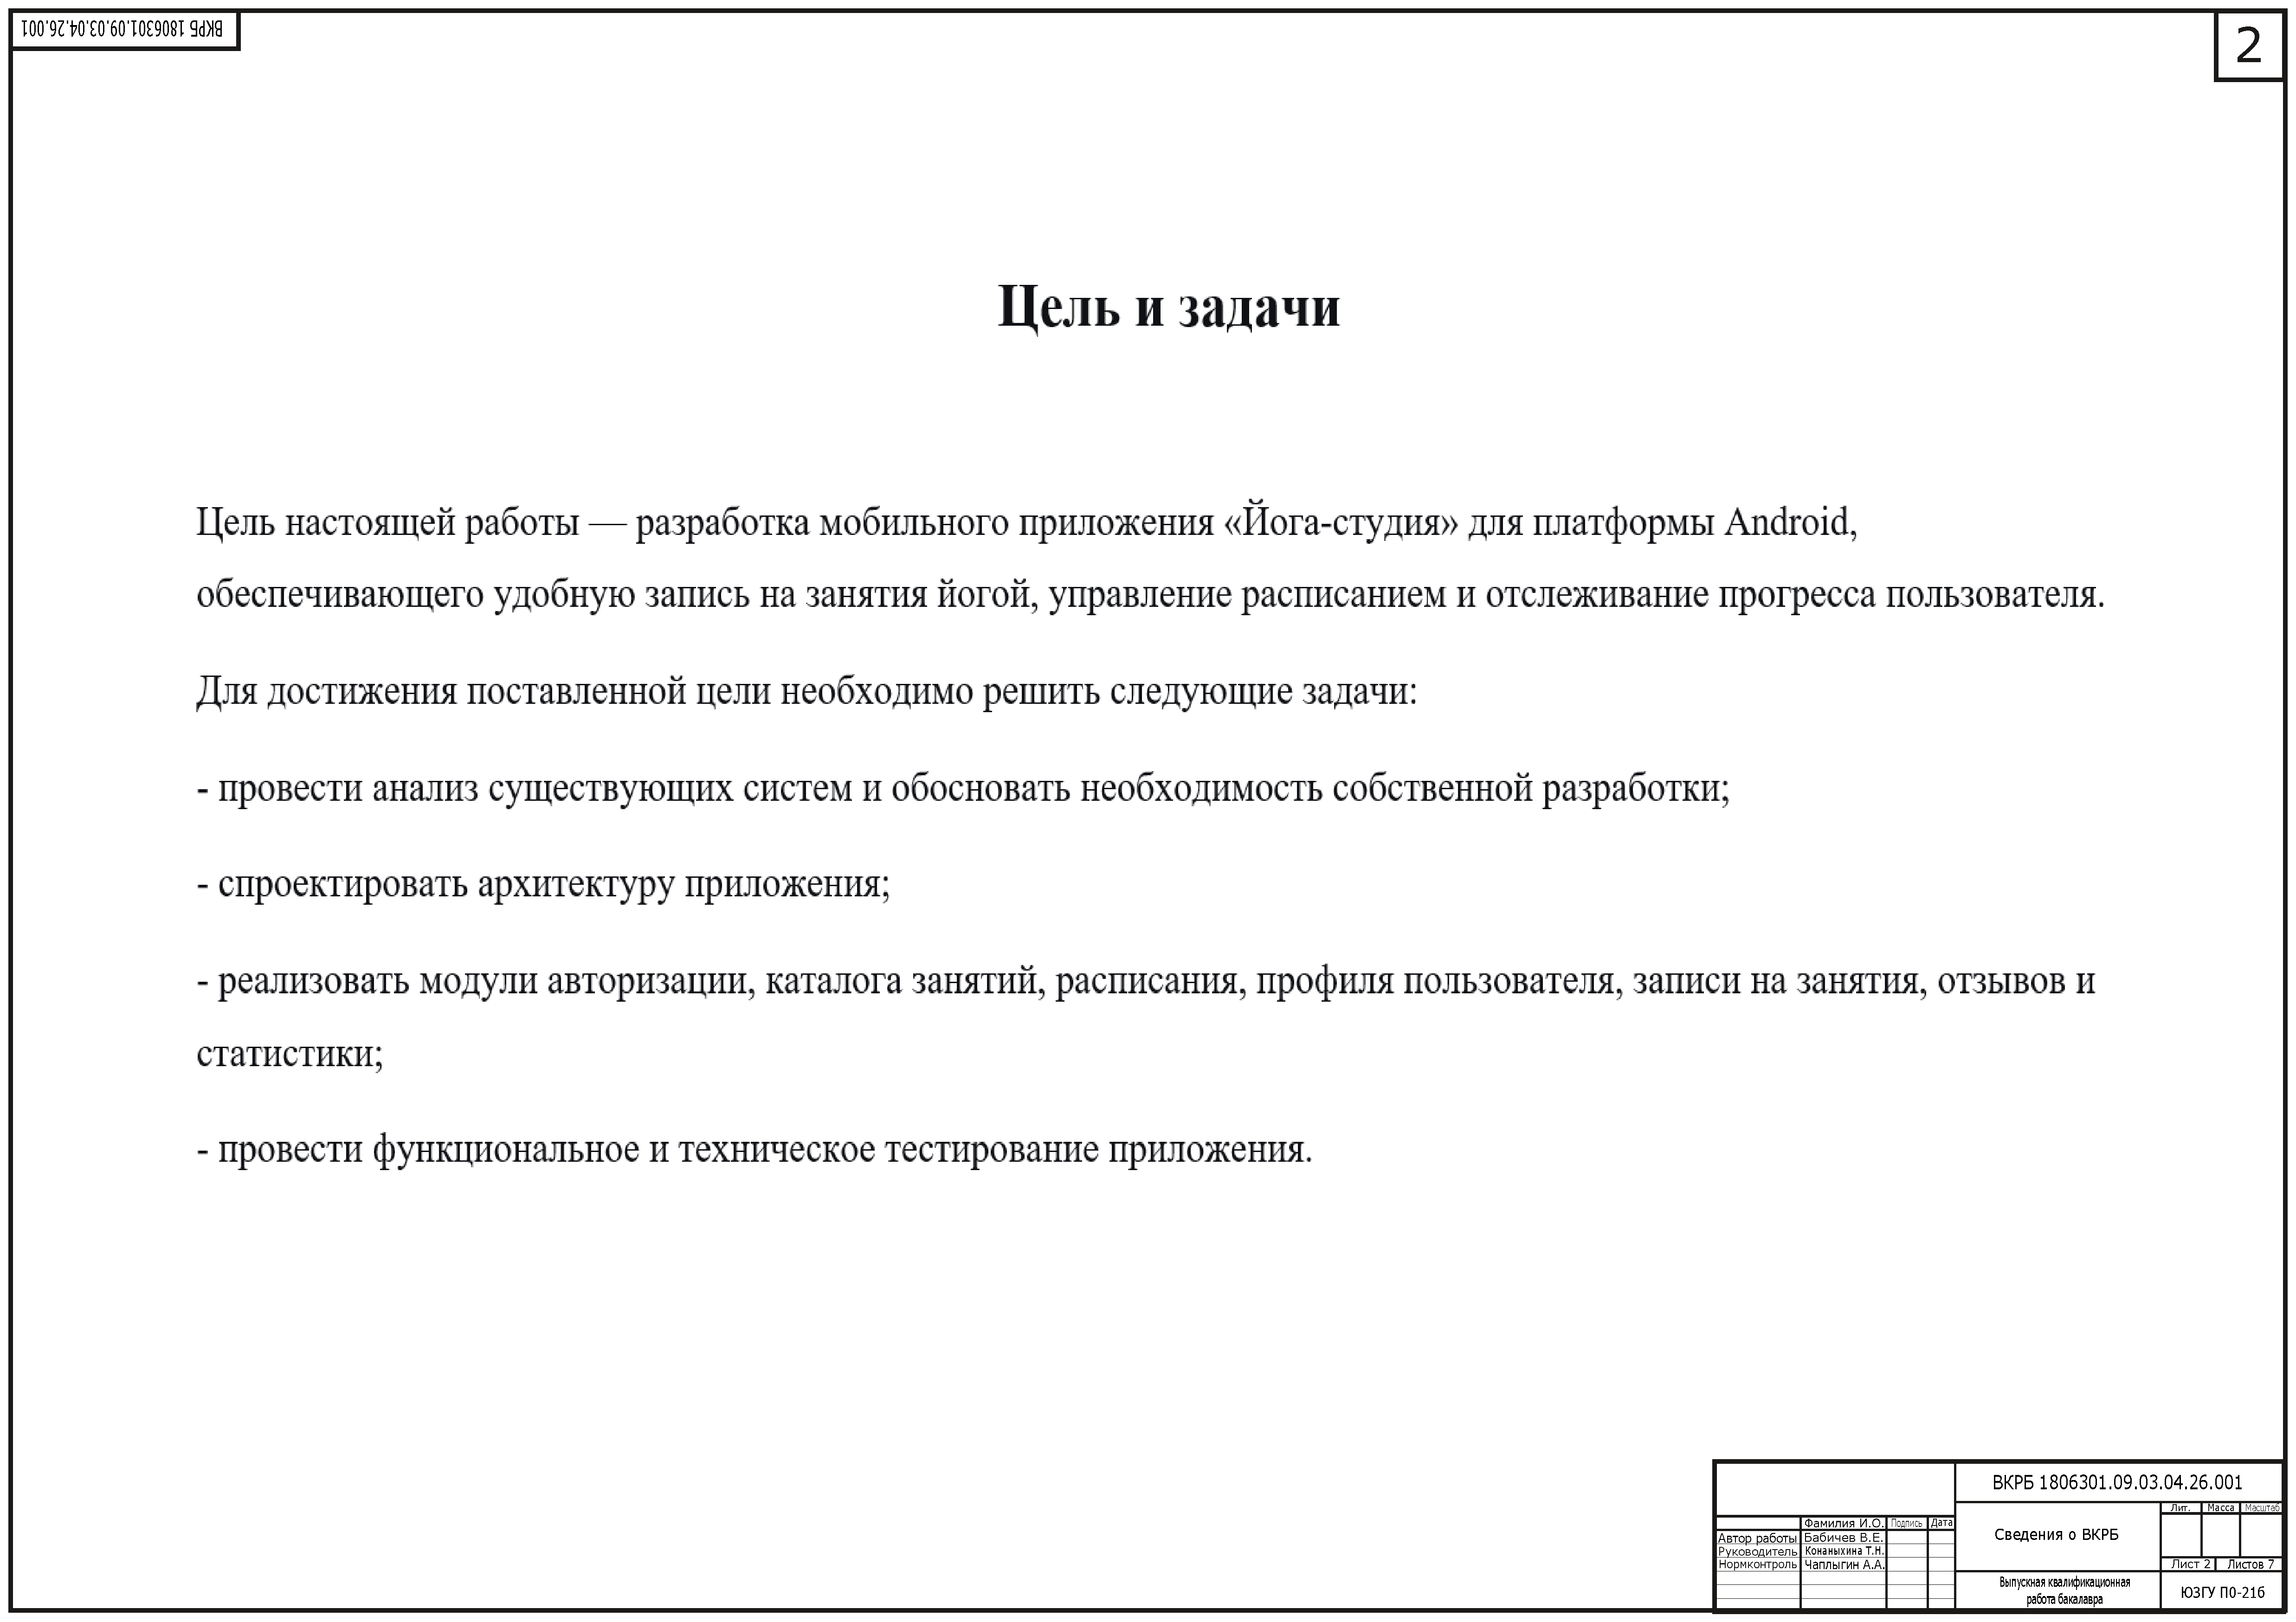
\includegraphics[width=0.82\linewidth]{images/Ramka_VKR2.eps}
		\заголовок{Цель и задачи разработки}
		\label{pl2:image}      
	\end{плакат}
	
	\begin{плакат}
		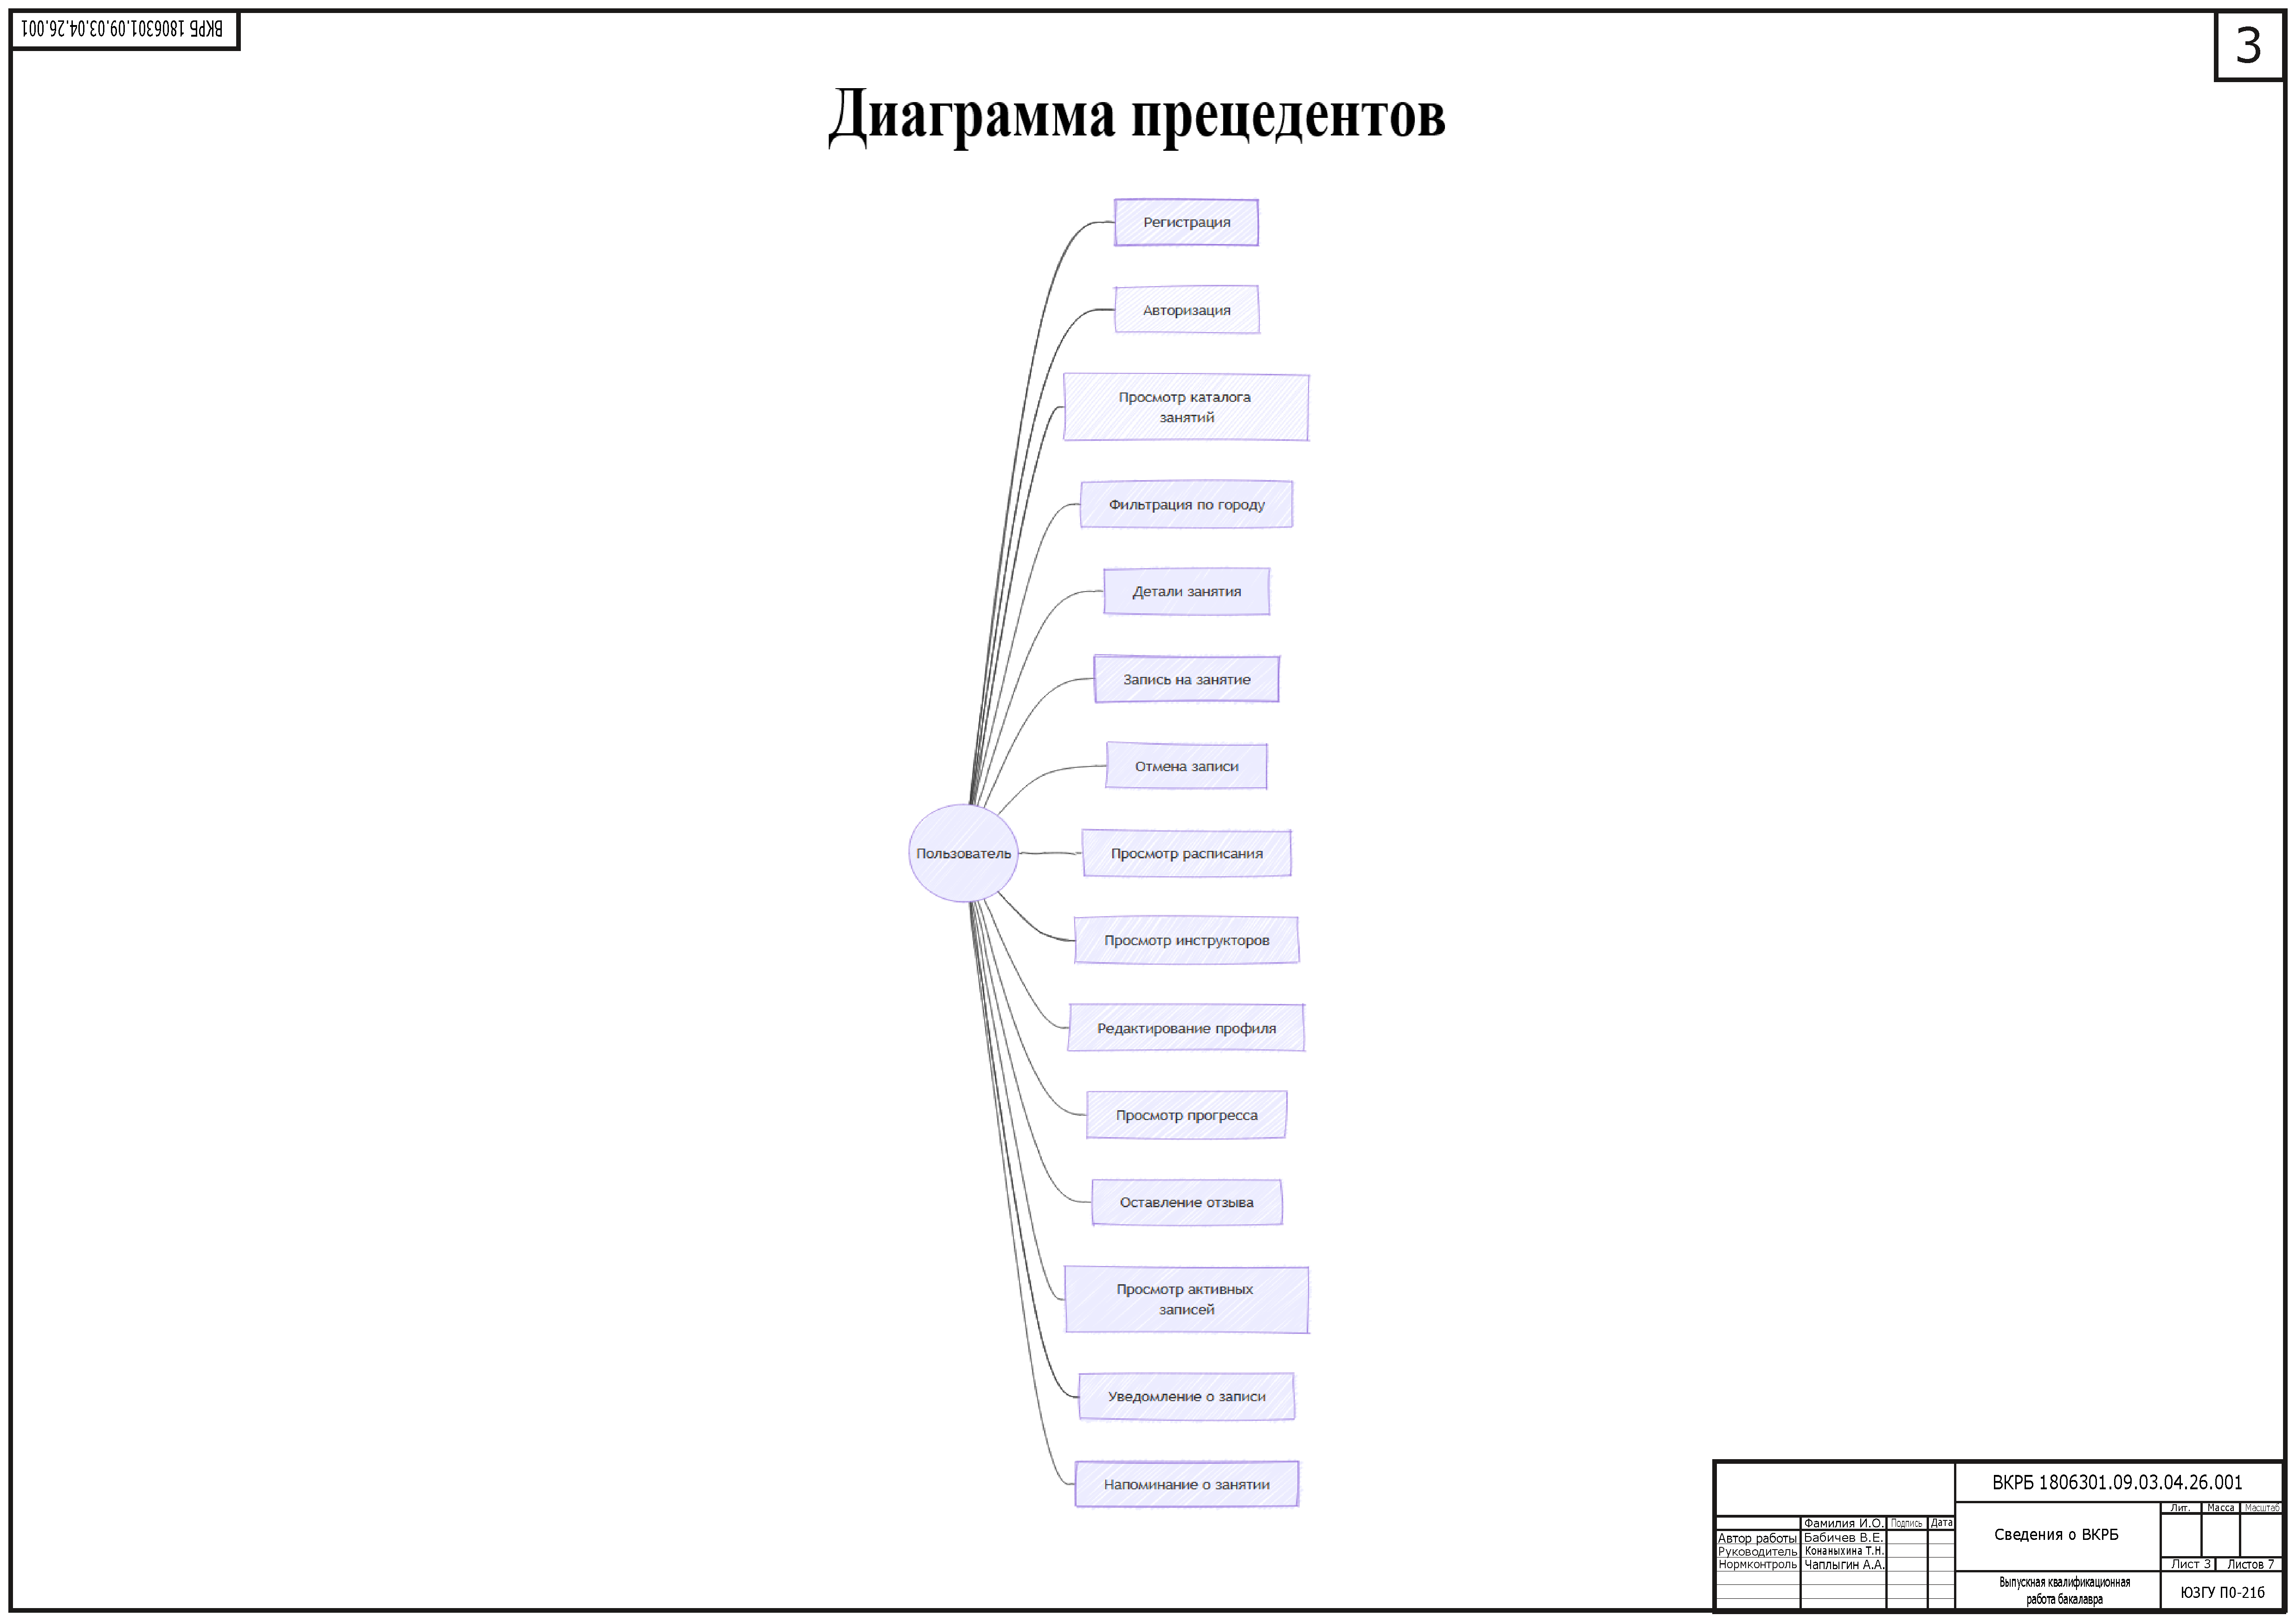
\includegraphics[width=0.82\linewidth]{images/Ramka_VKR3.eps}
		\заголовок{Архитектурная схема приложения}
		\label{pl3:image}      
	\end{плакат}
	
	\begin{плакат}
		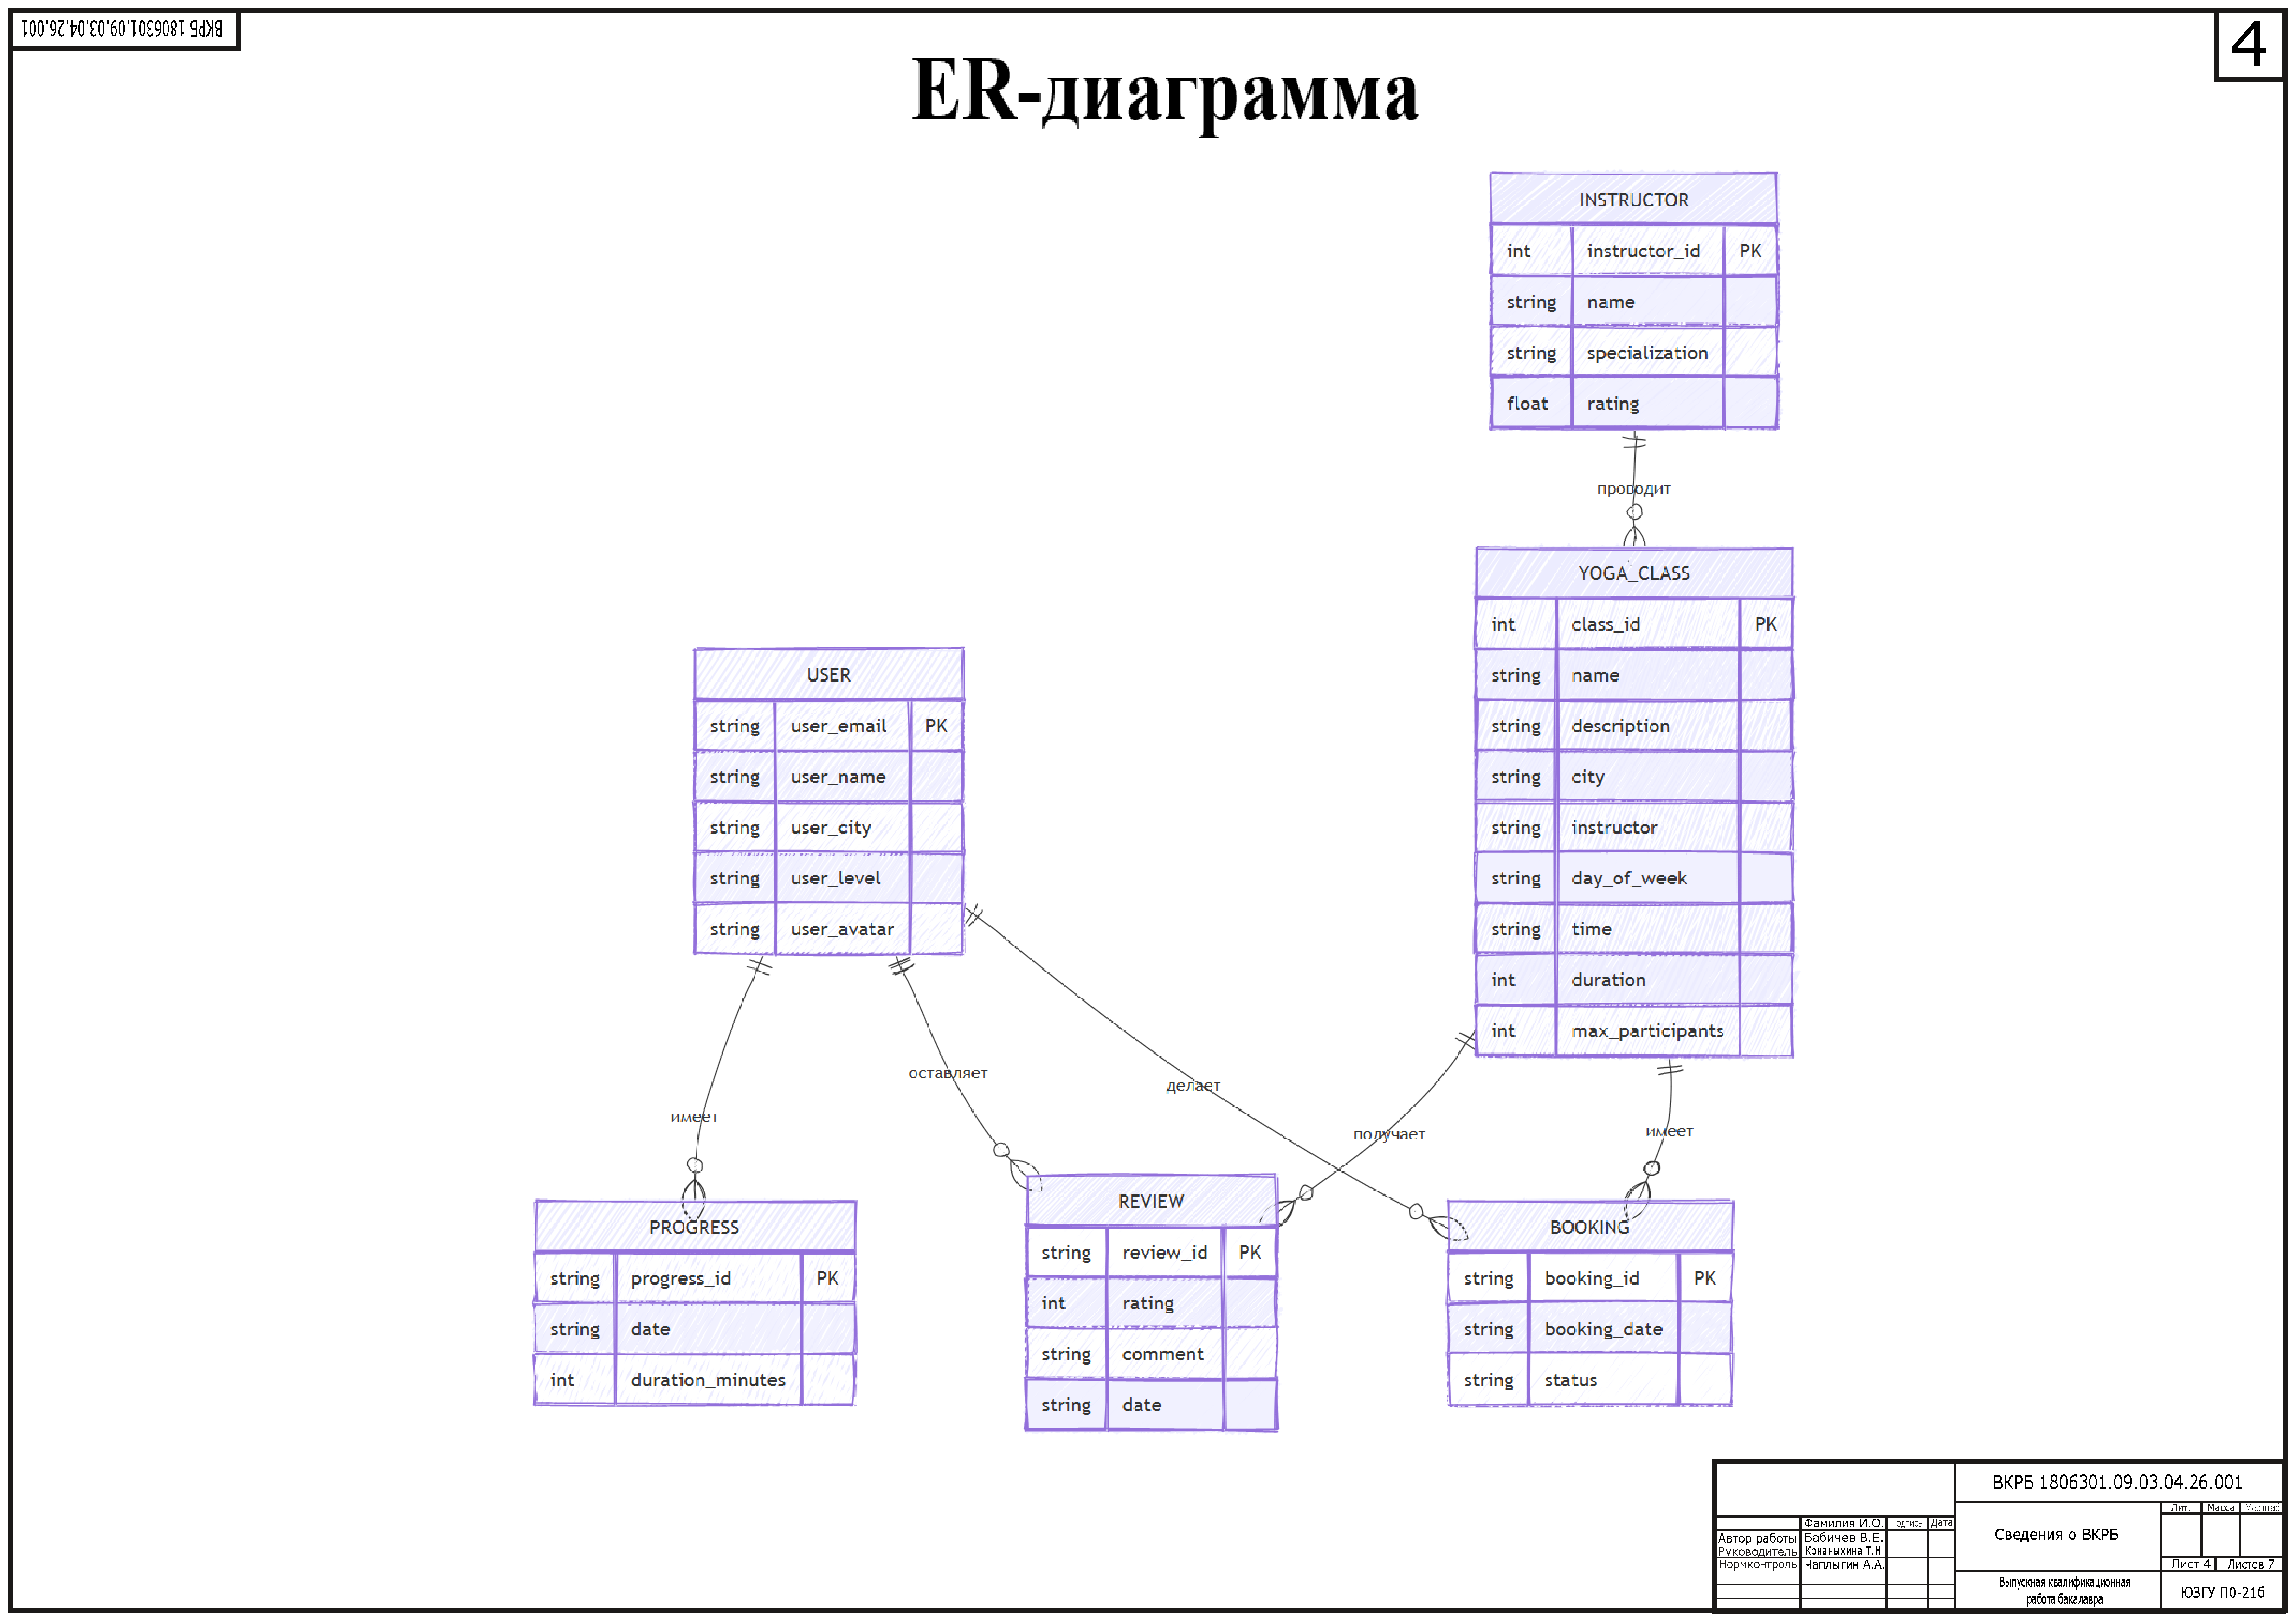
\includegraphics[width=0.82\linewidth]{images/Ramka_VKR4.eps}
		\заголовок{Диаграмма классов}
		\label{pl4:image}      
	\end{плакат}
	
	\begin{плакат}
		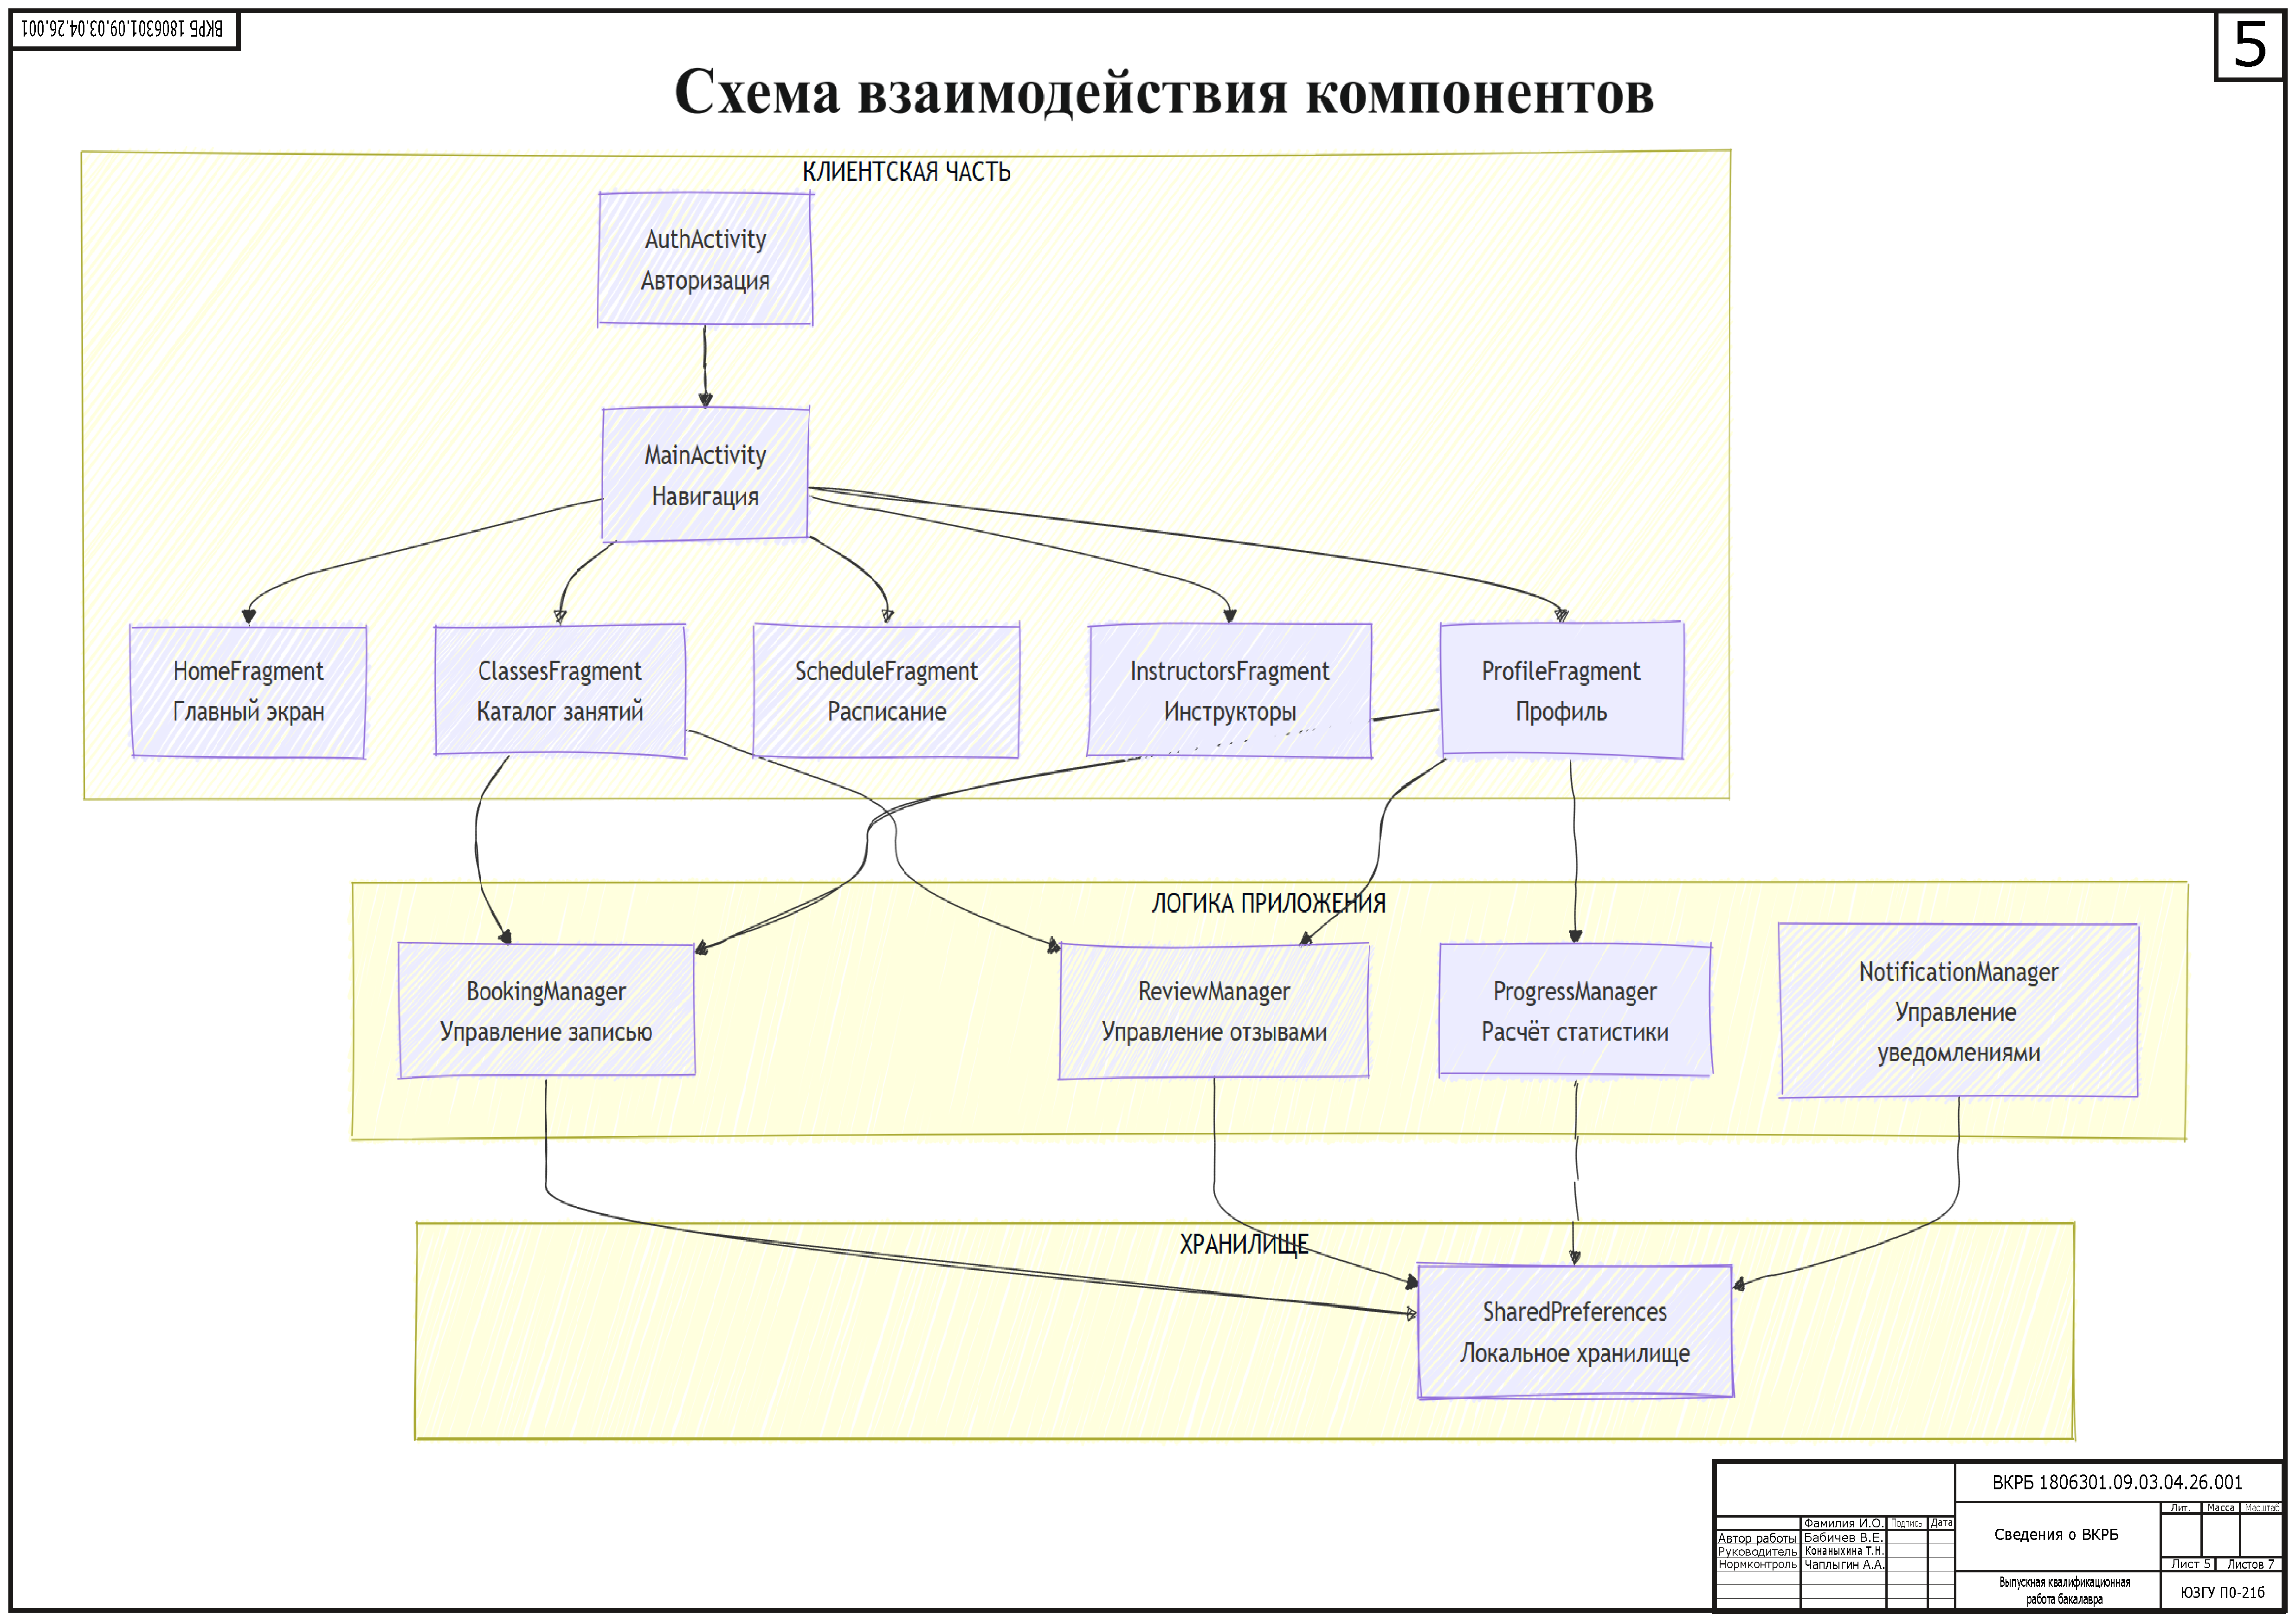
\includegraphics[width=0.82\linewidth]{images/Ramka_VKR5.eps}
		\заголовок{ER-диаграмма сущностей}
		\label{pl5:image}      
	\end{плакат}
	
	\begin{плакат}
		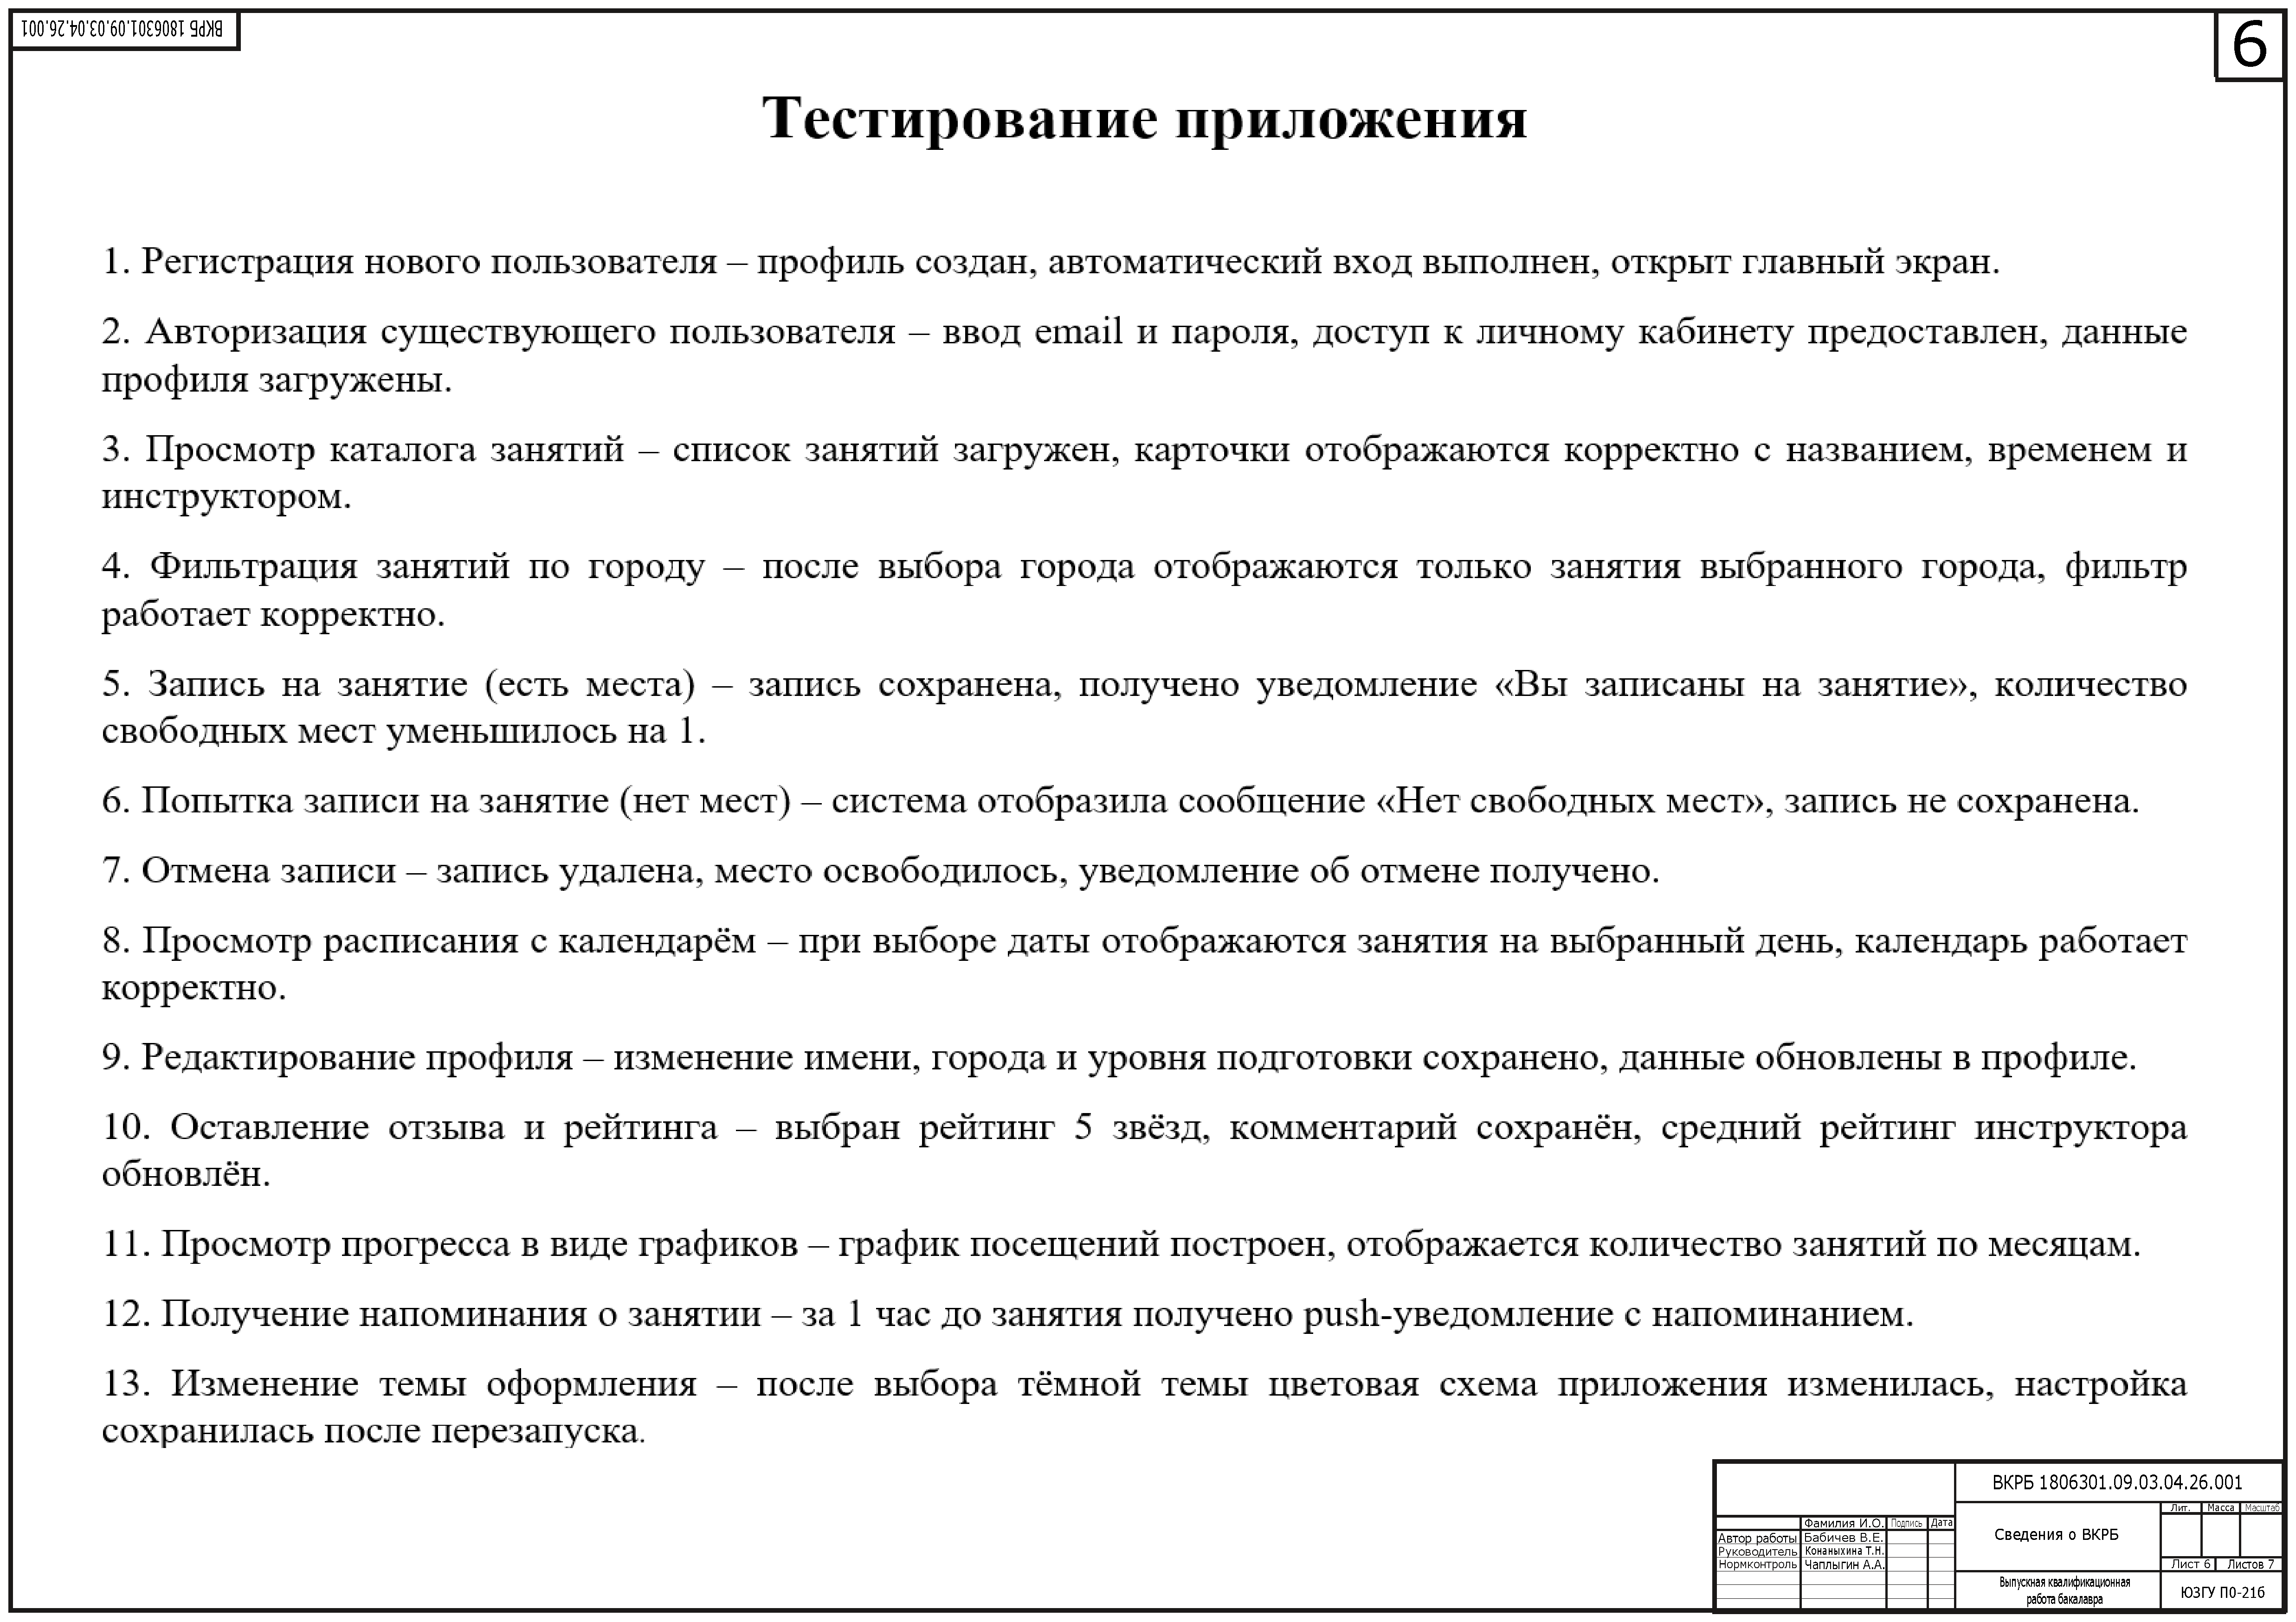
\includegraphics[width=0.82\linewidth]{images/Ramka_VKR6.eps}
		\заголовок{Диаграмма прецедентов}
		\label{pl6:image}      
	\end{плакат}
	
	\begin{плакат}
		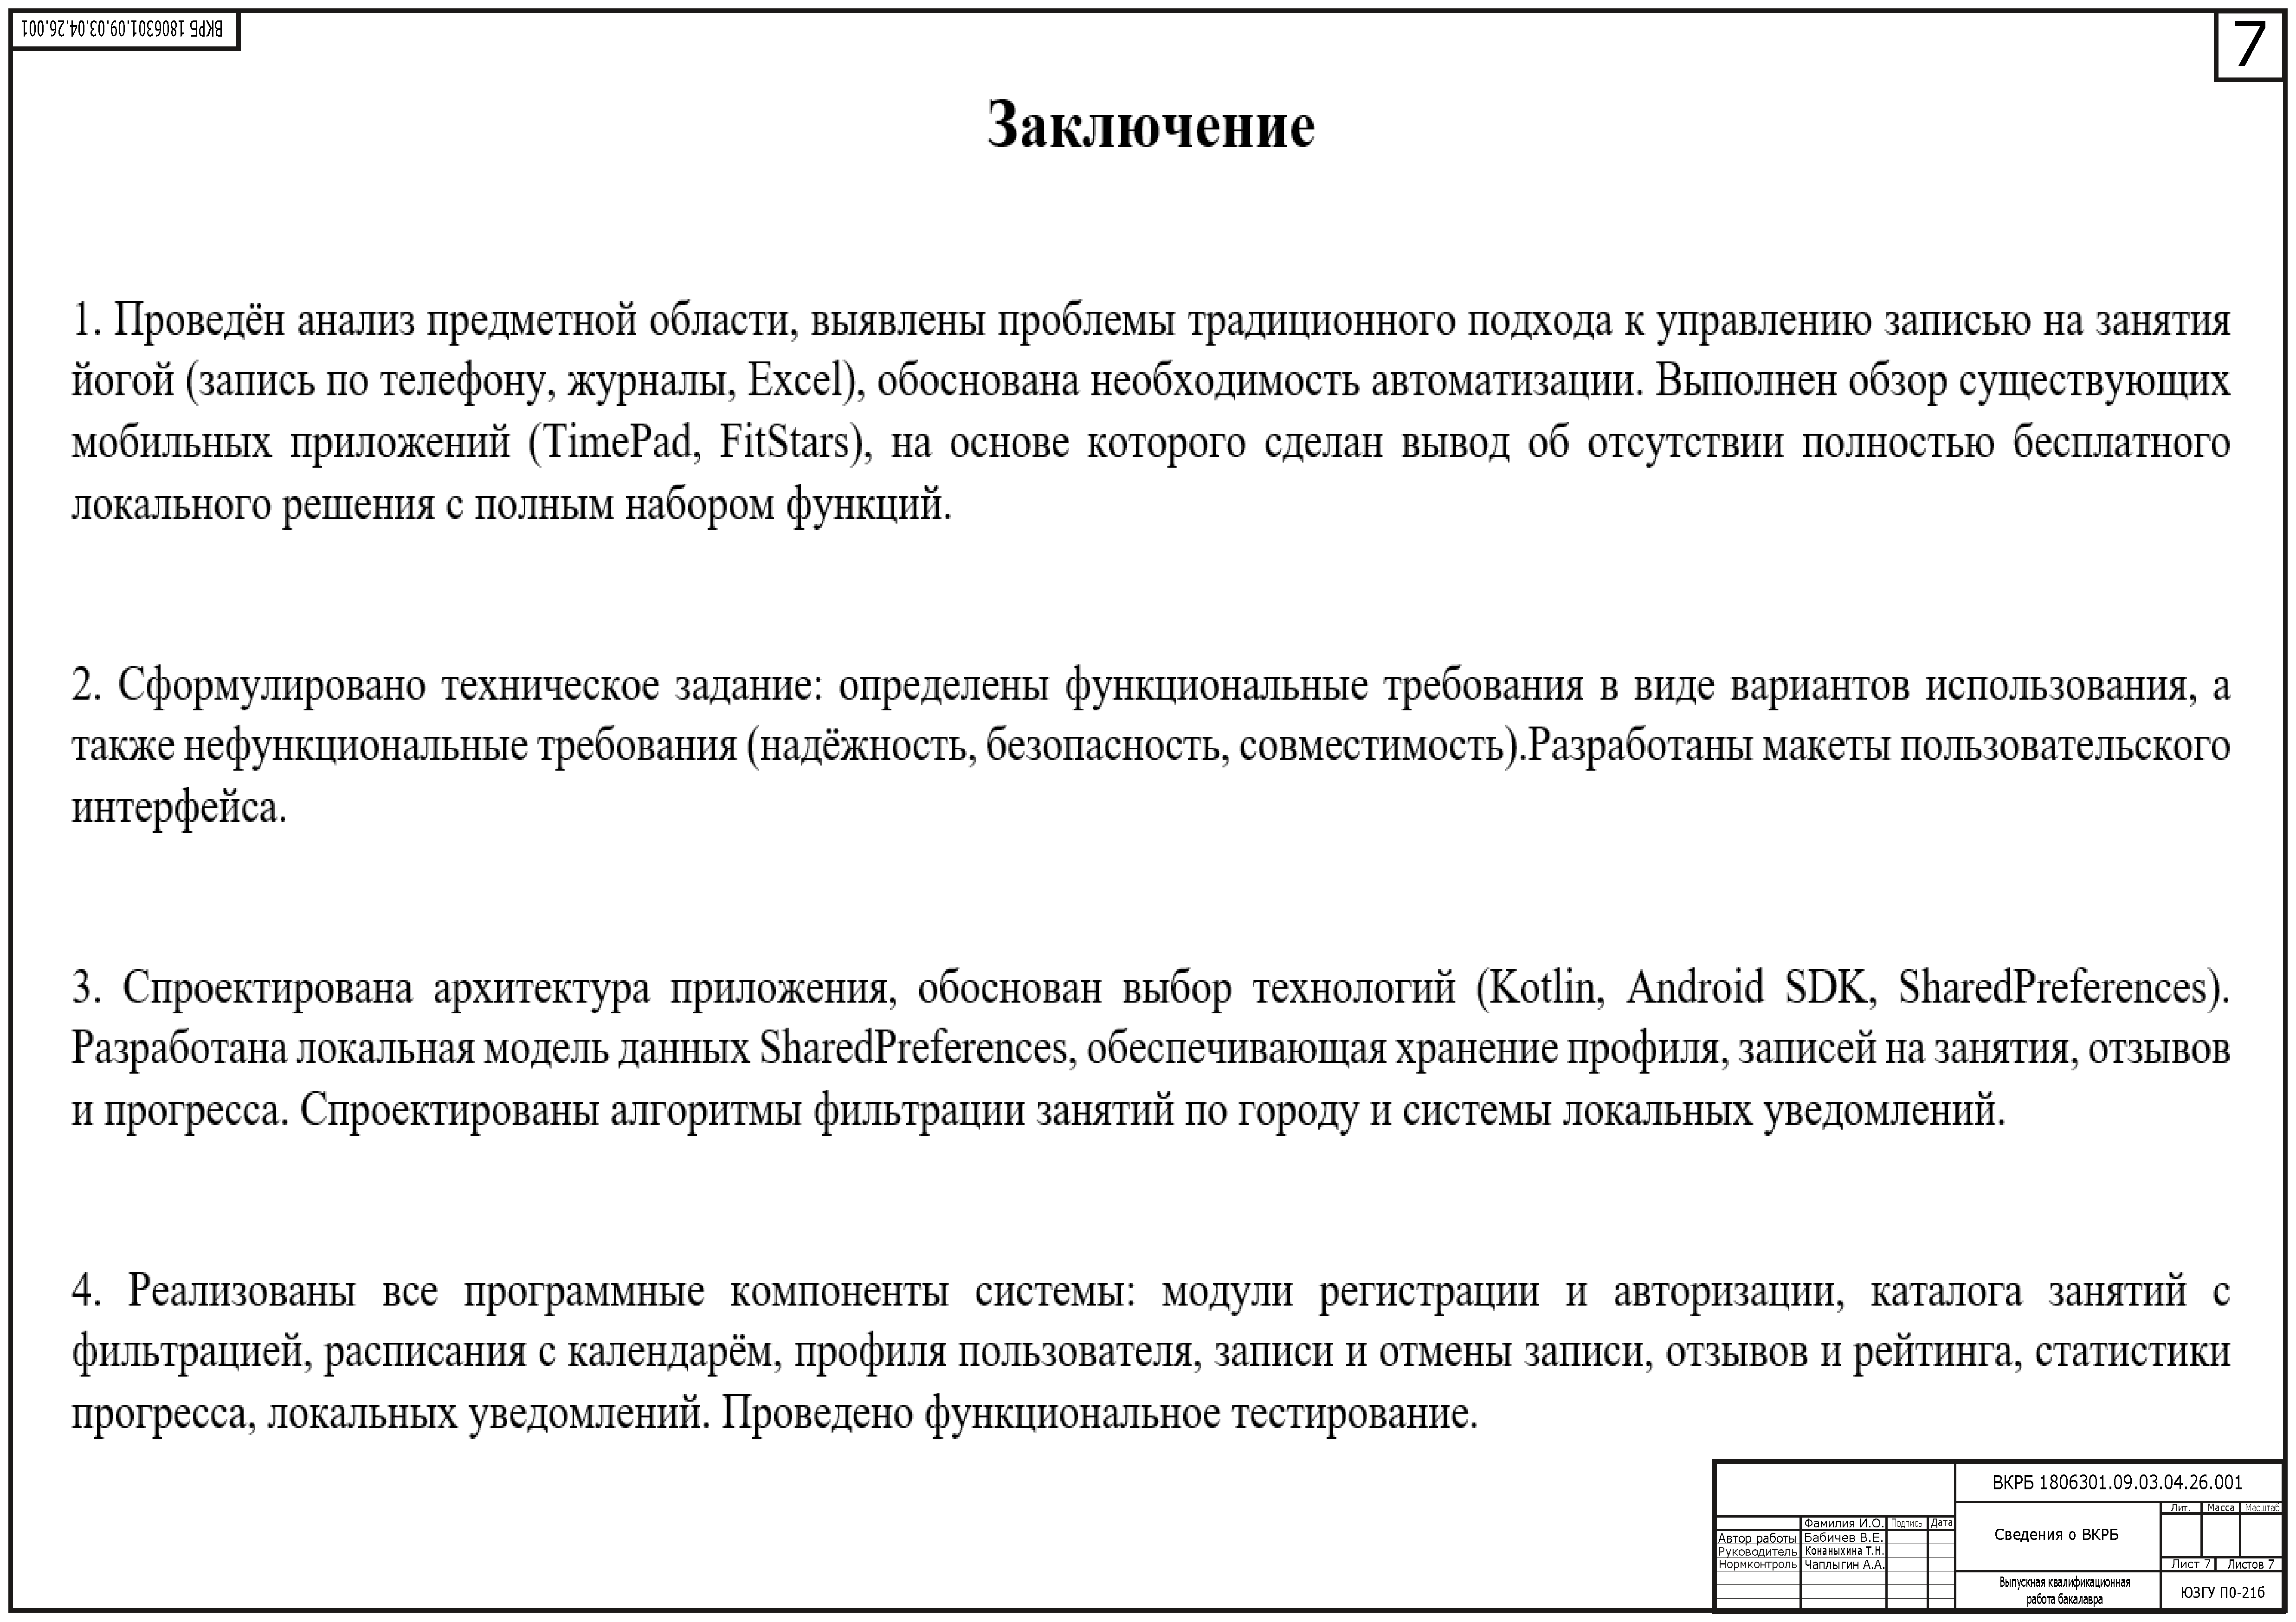
\includegraphics[width=0.82\linewidth]{images/Ramka_VKR7.eps}
		\заголовок{Заключение}
		\label{pl7:image}      
	\end{плакат}
	
\end{landscape}